\chapter{Experimentelle Grundlagen und Rahmenbedingungen}
    Forschungsgegenstand ist ein Reaktor, der im Rahmen des Verbundvorhabens $\mbox{SCOORE}$ (\textit{Synthesis gas from recycling of CO$_2$}) genutzt wurde. Ziel dieses Projekts ist es, eine CO$_2$-verbrauchende Synthesegasherstellung zu untersuchen und damit einen Beitrag zur Reduzierung der Treibhausgasemissionen in der chemischen Industrie zu leisten. 

    Das Vorhaben wird von der BASF~SE in Kooperation mit der Technischen Universität Bergakademie Freiberg durchgeführt und zielt darauf ab, eine großtechnisch umsetzbare Prozessführung für die nichtkatalytische Partialoxidation von Erdgas in einer CO$_2$-reichen Atmosphäre zu entwickeln \cite{Scoore_Enargus}.  
    \section{Aufbau der Versuchsanlage und des Reaktors}
        Der untersuchte Reaktor ist als zylindrischer Hochdruckreaktor mit feuerfester Ausmauerung ausgeführt und besitzt eine Gesamtlänge von ca. 1,5~m bei einem Innendurchmesser von 0,36~m. Die Anlage ist für Betriebsdrücke bis 70~bar und maximale Temperaturen bis 1400~°C ausgelegt. Der Brenner ist als Mehrloch-Mischbrenner ausgeführt, der eine homogene Mischung der eintretenden Ströme ermöglicht. Dieser Mischbrenner wird mit Wasser gekühlt. In Abbildung \ref{fig:reaktorgeometrie} ist der Aufbau des Brenners sowie des gesamten Reaktors dargestellt. 
        \begin{figure}[H]
            \centering
            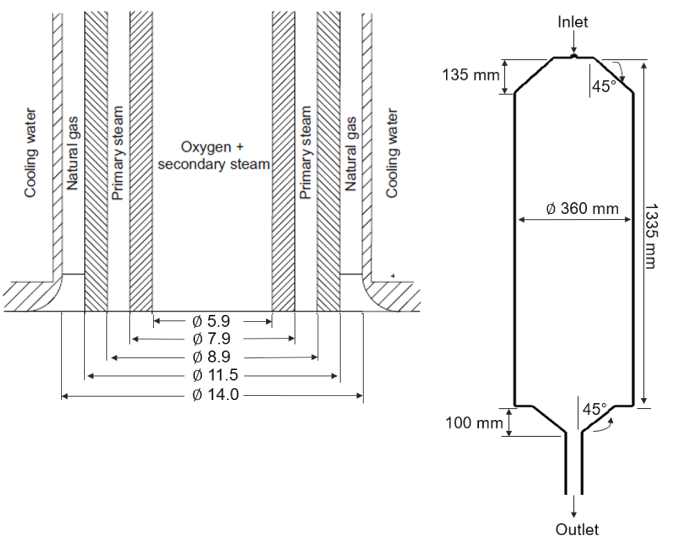
\includegraphics[width=0.6\linewidth]{img/sonstiges/Reaktorgeometrien.png}
            \caption{Geometrien des Reaktors sowie des Brenners}
            \label{fig:reaktorgeometrie}
        \end{figure}
    \section{Prozessbedingungen}
        Im Rahmen des Projekts wird der Prozess in zwei Varianten untersucht, um den Einfluss einer gezielten CO\textsubscript{2}-Zugabe auf die Reaktionsführung der nicht-katalytischen Hochdruck-Partialoxidation (HP-POx) von Erdgas systematisch zu bewerten. 
        
        Die erste Variante dient als Referenzprozess und beschreibt die konventionelle HP-POx von Erdgas unter Standardbedingungen ohne zusätzliche Zugabe von CO\textsubscript{2}. Dieser Fall repräsentiert den etablierten industriellen Prozess, bei dem Methan mit Sauerstoff und Wasserdampf unter stöchiometrisch limitierter Sauerstoffzufuhr zu einem Kohlenmonoxid- und wasserstoffhaltigen Synthesegas umgesetzt wird. 
        
        In der zweiten Variante wird der Reaktionsverlauf unter vergleichbaren thermischen und stofflichen Betriebsbedingungen untersucht, jedoch mit einem zusätzlichen CO\textsubscript{2}-Feed im Zulauf. Durch die Einmischung von CO\textsubscript{2} verändert sich das lokale Reaktionsgleichgewicht sowie die Temperaturführung im Reaktor, wodurch sich sowohl kinetische als auch thermodynamische Effekte ergeben. 
        
        Der Vergleich beider Prozessführungen erlaubt Rückschlüsse auf den Einfluss des CO\textsubscript{2}-Gehalts auf die chemische Umwandlung der Reaktanden sowie die Zusammensetzung des Produktgases. Darüber hinaus wird untersucht, inwieweit die CO\textsubscript{2}-Zugabe zur Reduktion der Netto-CO\textsubscript{2}-Emissionen beiträgt und welche Anpassungen an Betriebsparametern für eine stabile Prozessführung erforderlich sind.  
        
        In Tabelle \ref{tab:rahmenbedingungen_versuche} sind die wesentlichen Prozessparameter und Betriebsbedingungen der beiden Fälle zusammengefasst. Es ist ersichtlich, dass bei der CO\textsubscript{2}-Variante ein zusätzlicher Stoffstrom von etwa 196~kg/h Kohlenstoffdioxid in den Reaktor eingespeist wurde, während die übrigen Einsatzströme in Temperatur und Massenstrom nur geringfügig voneinander abweichen. Der Reaktor selbst weist ein Volumen von  134~Litern auf und wird unter stationären Bedingungen betrieben, wobei ein konstanter Wandwärmeverlust von etwa 30~kW berücksichtigt wird.
        
        \begin{table}[H]
            \centering
            \caption{Vergleich der Prozessfälle \cite{gonzales}}
            \label{tab:rahmenbedingungen_versuche}
            \begin{tabular}{llll}
            \toprule
            \textbf{Variablen} & & \textbf{Fall 1} & \textbf{Fall 2} \\
            \midrule
            \textbf{1. Erdgas} & Temperatur [°C] & 66,6 & 67,5 \\
                               & Massenstrom [kg/h] & 182,4 & 153,3 \\
            \midrule
            \textbf{2. Kohlenstoffdioxid} & Temperatur [°C] & -- & 67,5 \\
                                     & Massenstrom [kg/h] & 0 & 196,4 \\
            \midrule
            \textbf{3. Sauerstoff} & Temperatur [°C] & 231,9 & 231,2 \\
                                   & Massenstrom [kg/h] & 252,2 & 246,9 \\
            \midrule
            \textbf{4. Dampf} & Temperatur [°C] & 353,4 & 353,4 \\
                              & Massenstrom [kg/h] & 38,7 & 39,4 \\
            \midrule
            Wandwärmeverlust [kW] & & 30 & 30 \\
            Reaktorvolumen [L] & & 134 & 134 \\
            Druck [bar] && 47 & 47\\
            \midrule
            \textbf{Bemerkung} & & Referenz & CO\textsubscript{2}-Zugabe \\
            \bottomrule
            \end{tabular}
        \end{table}
        
    \section{Messverfahren und Messwerte}
        Entlang der Reaktorlängsachse sind mehrere Thermoelemente installiert, die die axiale Temperaturverteilung im Reaktor ermitteln. Zusätzlich sind Druck- und Massenstromsensoren in die Zuleitungen integriert, um die Prozessbedingungen konstant überwachen zu können. Das Produktgas wird am Reaktorausgang über eine gekühlte Probenahmeeinheit entnommen und anschließend gasanalytisch untersucht, wobei insbesondere die Volumenanteile von Wasserstoff, Kohlenstoffmonoxid, Kohlenstoffdioxid, Methan und Wasserdampf bestimmt werden \cite{RICHTER2015110}. Abbildung \ref{fig:erweiterungen_messpunkte} zeigt die Positionen der relevanten Thermoelemente. 
        \begin{figure}[H]
            \centering
            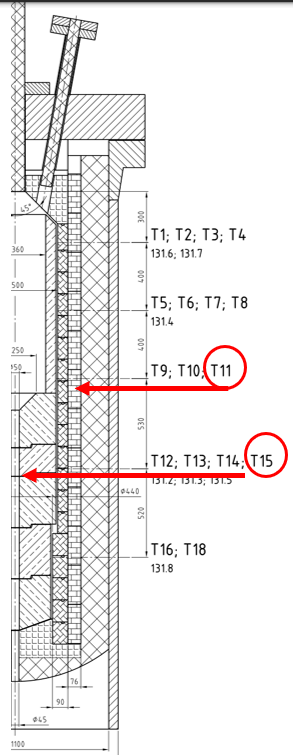
\includegraphics[width=0.2\linewidth]{img/Erweiterungen/Messpunkte.png}
            \caption{Messpunkte im Reaktor \cite{gonzales}}
            \label{fig:erweiterungen_messpunkte}
        \end{figure}
        Um die stofflichen Zusammensetzungen zu ermitteln, werden Infrarot-Absorptions\-spek\-troskopie (NDIR) und Wärmeleitfähigkeitsmessung (TCD) eingesetzt. Die ermittelten Daten der Zusammensetzung des Synthesegases und die Temperaturen beider Prozessbedingungen sind in Tabelle \ref{tab:messwerte} dargestellt. 
        \begin{table}[H]
            \centering
            \caption{Experimentelle Ergebnisse der Synthesegaszusammensetzungen sowie der Temperaturmessungen und Massenströme beider Betriebsweisen \cite{gonzales}}
            \label{tab:messwerte}
            \begin{tabular}{l l c c}
            \toprule
             & \textbf{Einheit} & \textbf{Fall 1 (Referenz)} & \textbf{Fall 2 (CO\textsubscript{2}-Zugabe)} \\
            \midrule
            Synthesegas (nass) & kg/s & 0{,}13 & 0{,}18 \\
            Temperatur Austritt & °C & (1300)\textsuperscript{*} & (1342)\textsuperscript{*} \\
            Temperatur T102.11 & °C & 1407{,}4 & 1411{,}4 \\
            Temperatur T102.15 & °C & 1351{,}9 & 1371{,}6 \\
            \midrule
            H\textsubscript{2} & Vol.-\% trocken & 0{,}599 & 0{,}416 \\
            CO & Vol.-\% trocken & 0{,}341 & 0{,}416 \\
            CH\textsubscript{4} & Vol.-\% trocken & 0{,}007 & 0{,}0012 \\
            CO\textsubscript{2} & Vol.-\% trocken & 0{,}048 & 0{,}151 \\
            \midrule
            H\textsubscript{2}/CO & – & 1{,}751 & 0{,}981 \\
            \bottomrule
            \end{tabular}
            \footnotesize{*~Werte in Klammern wurden mit \textit{Aspen Plus} berechnet und stellen keinen Experimentalwert dar.}
        \end{table}
    \section{Vorbetrachtungen}
        \label{sec:vorbetrachtungen}
        Zur Vorbereitung der Modellierungsarbeiten liegen bereits umfangreiche CFD-Analysen sowie ein darauf basierendes komplexes Reaktornetzwerk-Modell (ROM) aus dem Projekt SCOORE vor. Diese Untersuchungen bilden die Grundlage für das Verständnis der Strömungs- und Reaktionsvorgänge innerhalb des betrachteten POx-Reaktors \cite{gonzales}. 
        
        %Die CFD-Simulationen wurden unter stationären Bedingungen mit detaillierter Berücksichtigung der Strömungs- und Temperaturfelder durchgeführt. Auf Basis dieser Ergebnisse erfolgte eine Segmentierung des Reaktors in charakteristische Zonen, die durch idealisierte Reaktoren beschrieben werden können. 
        %In Abbildung \ref{fig:reaktorsegmentierung} ist die CFD-basierte Segmentierung des Reaktors dargestellt, aus der das bestehende Netzwerk aus Perfectly Stirred Reactors (PSR) und Plug Flow Reactors (PFR) abgeleitet wurde.
        Die CFD-Simulation wurde unter stationären Bedingungen mit detaillierter Berücksichtigung der Strömungs- und Temperaturfelder durchgeführt. Dabei konnte der Reaktor in charakteristische Strömungszonen segmentiert werden, die sich untereinander durch verschiedene Reaktions- und Mischcharakteristiken auszeichnen. Auf Basis dieser Simulation erfolgte die konzeptionelle Erstellung des komplexen ROMs, das PFR- und PSR- Elemente enthält. Diese Segmentierung ermöglicht eine deutliche Vereinfachung der Berechnung dieses Reaktors. 
        
        \begin{figure}[H]
            \centering
            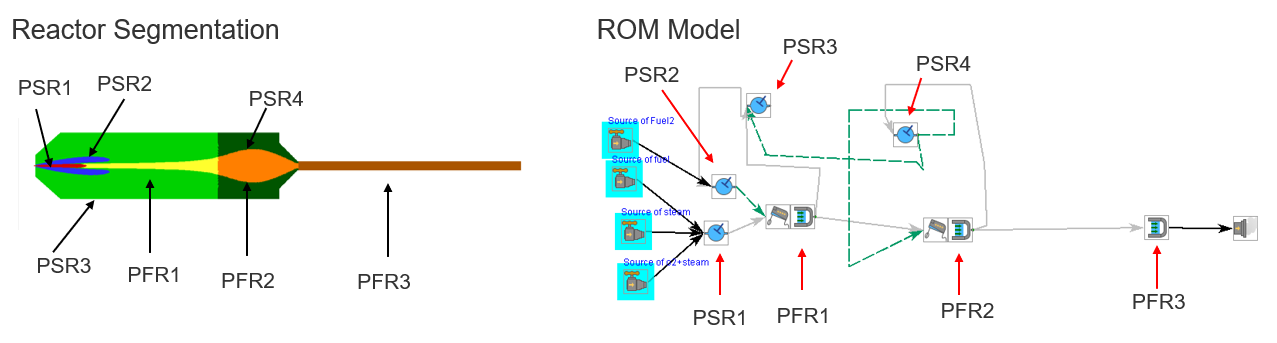
\includegraphics[width=1\linewidth]{img/sonstiges/Reactor Segmentation.png}
            \caption{Reaktorsegmentierung und komplexes ROM auf Basis einer CFD-Simulation \cite{gonzales}}
            \label{fig:reaktorsegmentierung}
        \end{figure}
        